% !Mode:: "TeX:UTF-8"

\chapter{项目测试}

\section{前端测试}

根据UI效果图进行UI测试
\begin{enumerate}
\item 观察APP的用户界面(如菜单、对话框、窗口和其它可规控件)是否符合UI稿
\item 不同的连接页面之间导航链接是否有效,是否跳转是否正确
\item 输入框说明文字的内容与产品需求一致
\item 某页无数据时、断网时、有网但接口异常时的状态页是否和UI一致
\end{enumerate}

\section{接口测试}
\begin{enumerate}
\item Get,post发送和返回是否请求正常
\item 查看请求参数和返回参数结果是否正常
\end{enumerate}
(测试接口工具:postman)

\section{功能测试}
业务功能流程如图\ref{fig:prog}所示
\begin{figure}[htbp]
    \centering
    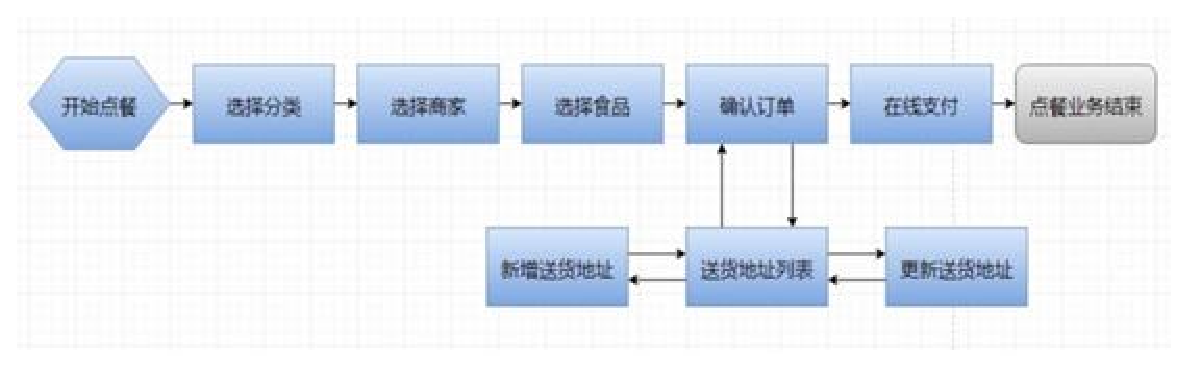
\includegraphics[width=0.8\textwidth]{progress}
    \caption{点餐业务流程图}\label{fig:prog}
    \vspace{\baselineskip}
    \end{figure}

    
\begin{verbatim}
    功能测试在前后端连接之后,主要按照点餐业务流程图的功能依次进行测试,依据编写的功能测试用例进行软件功能的测试。通过观察实行操作后页面的显示,提示框的弹出以及数据库内容的改变来判断功能是否完成。
    
\end{verbatim}